%NEURAL PRESY ;)

%----------------------------------------------------------------------------------------
%   PACKAGES AND THEMES
%----------------------------------------------------------------------------------------

\documentclass{beamer}

\mode<presentation> {

% The Beamer class comes with a number of default slide themes
% which change the colors and layouts of slides. Below this is a list
% of all the themes, uncomment each in turn to see what they look like.

%\usetheme{default}
%\usetheme{AnnArbor}
%\usetheme{Antibes}
%\usetheme{Bergen}
\usetheme{Berkeley}
%\usetheme{Berlin}
%\usetheme{Boadilla}
%\usetheme{CambridgeUS}
%\usetheme{Copenhagen}
%\usetheme{Darmstadt}
%\usetheme{Dresden}
%\usetheme{Frankfurt}
%\usetheme{Goettingen}
%\usetheme{Hannover}
%\usetheme{Ilmenau}
%\usetheme{JuanLesPins}
%\usetheme{Luebeck}
%\usetheme{Madrid}
%\usetheme{Malmoe}
%\usetheme{Marburg}
%\usetheme{Montpellier}
%\usetheme{PaloAlto}
%\usetheme{Pittsburgh}
%\usetheme{Rochester}
%\usetheme{Singapore}
%\usetheme{Szeged}
%\usetheme{Warsaw}

% As well as themes, the Beamer class has a number of color themes
% for any slide theme. Uncomment each of these in turn to see how it
% changes the colors of your current slide theme.

%\usecolortheme{albatross}
%\usecolortheme{beaver}
%\usecolortheme{beetle}
%\usecolortheme{crane}
%\usecolortheme{dolphin}
%\usecolortheme{dove}
%\usecolortheme{fly}
%\usecolortheme{lily}
%\usecolortheme{orchid}
%\usecolortheme{rose}
%\usecolortheme{seagull}
%\usecolortheme{seahorse}
%\usecolortheme{whale}
%\usecolortheme{wolverine}

%\setbeamertemplate{footline} % To remove the footer line in all slides uncomment this line
%\setbeamertemplate{footline}[page number] % To replace the footer line in all slides with a simple slide count uncomment this line

%\setbeamertemplate{navigation symbols}{} % To remove the navigation symbols from the bottom of all slides uncomment this line
}

\usepackage{graphicx} % Allows including images
\graphicspath{ {images/} }
\usepackage{booktabs} % Allows the use of \toprule, \midrule and \bottomrule in tables

\def\layersep{2cm}
\usepackage{tikz}
%----------------------------------------------------------------------------------------
%   TITLE PAGE
%----------------------------------------------------------------------------------------

\title[Neural Networks Pt. 2]{Neural Networks Workshop: Training and Stochastic Gradient Descent}

\author[W.\,Guss \& P.\,Kuznetsov]
{%
  \texorpdfstring{
    \begin{columns}%[onlytextwidth]
      \column{.45\linewidth}
      \centering
      William Guss\\
      \href{mailto:wguss@berkeley.edu}{wguss@berkeley.edu}
      \column{.45\linewidth}
      \centering
      Phillip Kuznetsov\\
      \href{mailto:philkuz@berkeley.edu}{philkuz@berkeley.edu}
    \end{columns}
  }
  {William Guss \& Phillip Kuznetsov}
}
\institute[UCB]
{
University of California, Berkeley \\
Robotics @ Berkeley \\
}

\date{December 1, 2015} % Date, can be changed to a custom date

\begin{document}

\begin{frame}
\titlepage
\end{frame}

\begin{frame}

\begin{center}
\Huge Today we use and train Feed-Forward Artificial Neural Networks
\end{center}

\frametitle{Overview}
\tableofcontents
\end{frame}

%----------------------------------------------------------------------------------------
%   PRESENTATION SLIDES
%----------------------------------------------------------------------------------------

%------------------------------------------------
\section{Feed-Forward Neural Networks} % Sections can be created in order to organize your presentation into discrete blocks, all sections and subsections are automatically printed in the table of contents as an overview of the talk
%-----------------------------------------------

    \begin{frame}
        \frametitle{Perceptron Review}
        \begin{center}
            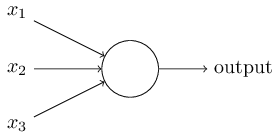
\includegraphics[scale=.3]{perceptron}
        \end{center}
        \begin{itemize}
        \item Perceptrons are neural computation units which make \emph{weighted} decisions:
        \begin{equation*}
            \begin{aligned}
                p(\pmb x) &= \left\{
                 \begin{array}l
                 1\ \text{if}\ \sum w_ix_i + b\geq 0\\
                 0\ \text{otherwise}
                \end{array}
                \right. \\
                &= \frac{\text{sign}\left(\sum w_ix_i + b\right) + 1}{2}
            \end{aligned}
        \end{equation*}
        \item Perceptrons are not powerful enough, as seen last time with XOR.
        \item What if we want real valued output for tasks like predicting
         the temparature or stock prices?
        \end{itemize}
    \end{frame}

    \begin{frame}
        \frametitle{Feedforward Neural Networks}
        [TODO: IMAGE OF FEED FORWARD NETWORK]
        \begin{itemize}
        \item Feedforward Artifical Neural Networks (ANNs) are the \emph{continuous}
        extensions of perceptrons.
        \item ANNs can have many layers and different nodes
         which are \emph{fully connected.}
       
         \item The intuition behind this model is that each neuron in the network
         makes a weighted decision like the perceptron. Many \emph{stacked} decisions
         allows for extremely complex logic.
        \end{itemize}
    \end{frame}

    \subsection{How They Work} % A subsection can be created just before a set of slides with a common theme to further break down your presentation into chunks



    \subsection{Universal Approximation (Briefly)}

\section{Training}

    \subsection{Nonconvex Optimization}
    \subsection{Error-Backpropagation}

\section{Deep Learning}


%------------------------------------------------

\begin{frame}
\frametitle{Blocks of Highlighted Text}
\begin{block}{Block 1}
Lorem ipsum dolor sit amet, consectetur adipiscing elit. Integer lectus nisl, ultricies in feugiat rutrum, porttitor sit amet augue. Aliquam ut tortor mauris. Sed volutpat ante purus, quis accumsan dolor.
\end{block}

\begin{block}{Block 2}
Pellentesque sed tellus purus. Class aptent taciti sociosqu ad litora torquent per conubia nostra, per inceptos himenaeos. Vestibulum quis magna at risus dictum tempor eu vitae velit.
\end{block}

\begin{block}{Block 3}
Suspendisse tincidunt sagittis gravida. Curabitur condimentum, enim sed venenatis rutrum, ipsum neque consectetur orci, sed blandit justo nisi ac lacus.
\end{block}
\end{frame}

%------------------------------------------------

\begin{frame}
\frametitle{Multiple Columns}
\begin{columns}[c] % The "c" option specifies centered vertical alignment while the "t" option is used for top vertical alignment

\column{.45\textwidth} % Left column and width
\textbf{Heading}
\begin{enumerate}
\item Statement
\item Explanation
\item Example
\end{enumerate}

\column{.5\textwidth} % Right column and width
Lorem ipsum dolor sit amet, consectetur adipiscing elit. Integer lectus nisl, ultricies in feugiat rutrum, porttitor sit amet augue. Aliquam ut tortor mauris. Sed volutpat ante purus, quis accumsan dolor.

\end{columns}
\end{frame}


\begin{frame}
\frametitle{Table}
\begin{table}
\begin{tabular}{l l l}
\toprule
\textbf{Treatments} & \textbf{Response 1} & \textbf{Response 2}\\
\midrule
Treatment 1 & 0.0003262 & 0.562 \\
Treatment 2 & 0.0015681 & 0.910 \\
Treatment 3 & 0.0009271 & 0.296 \\
\bottomrule
\end{tabular}
\caption{Table caption}
\end{table}
\end{frame}

%------------------------------------------------

\begin{frame}
\frametitle{Theorem}
\begin{theorem}[Mass--energy equivalence]
$E = mc^2$
\end{theorem}
\end{frame}

%------------------------------------------------

\begin{frame}[fragile] % Need to use the fragile option when verbatim is used in the slide
\frametitle{Verbatim}
\begin{example}[Theorem Slide Code]
\begin{verbatim}
\begin{frame}
\frametitle{Theorem}
\begin{theorem}[Mass--energy equivalence]
$E = mc^2$
\end{theorem}
\end{frame}\end{verbatim}
\end{example}
\end{frame}

%------------------------------------------------

\begin{frame}
\frametitle{Figure}
  \begin{figure}
  \centering
  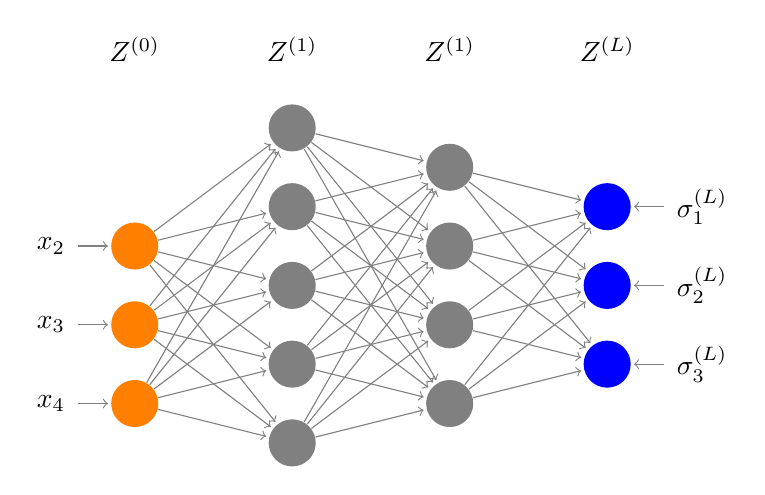
\begin{tikzpicture}[shorten >=1pt,->,draw=black!50, node distance=\layersep]
      \tikzstyle{every pin edge}=[<-,shorten <=1pt]
      \tikzstyle{neuron}=[circle,fill=black!25,minimum size=17pt,inner sep=0pt]
      \tikzstyle{input neuron}=[neuron, fill=orange];
      \tikzstyle{output neuron}=[neuron, fill=blue!100];
      \tikzstyle{hidden neuron}=[neuron, fill=black!50];
      \tikzstyle{annot} = [text width=4em, text centered]

      % Draw the input layer nodes
      \foreach \name / \y in {2,...,4}
      % This is the same as writing \foreach \name / \y in {1/1,2/2,3/3,4/4}
          \node[input neuron, pin=left: \(x_\y\)] (I-\name) at (0,-\y) {};

      % Draw the hidden layer nodes
      \foreach \name / \y in {1,...,5}
          \path[yshift=0.5cm]
              node[hidden neuron] (H1-\name) at (\layersep,-\y cm) {};
              
       \foreach \name / \y in {1,...,4}
          \path[yshift=0.5cm]
              node[hidden neuron] (H2-\name) at (2*\layersep,-0.5cm -\y cm) {};

      % Draw the hidden layer nodes
      \foreach \name / \y in {1,...,3}
          \path[yshift=0.5cm]
              node[output neuron, pin=right:\(\sigma_{\name}^{(L)}\)] (O-\name) at (3*\layersep,-1cm -\y cm) {};


      % Connect every node in the input layer with every node in the
      % hidden layer.
      \foreach \source in {2,...,4}
          \foreach \dest in {1,...,5}
              \path (I-\source) edge (H1-\dest);

      % Connect every node in the hidden layer with the output layer
      
          \foreach \source in {1,...,5}
          \foreach \dest in {1,...,4}
          \path (H1-\source) edge (H2-\dest);
      \foreach \source in {1,...,4}
          \foreach \dest in {1,...,3}
          \path (H2-\source) edge (O-\dest);

      % Annotate the layers
      \node[annot,above of=H1-1, node distance=1cm] (hl) {\(Z^{(1)}\)};
      \node[annot,left of=hl] {\(Z^{(0)}\)};
      \node[annot,right of=hl] {\(Z^{(1)}\)};
      \node[annot,above of=O-1, node distance=2cm] (ol) {\(Z^{(L)}\)};
  \end{tikzpicture}
    \caption[An example of a feed-forward ANN]{An example of a feed-forward ANN,  \(\mathcal{N}\) with four layers.}
  \end{figure}

\end{frame}

%------------------------------------------------

\begin{frame}[fragile] % Need to use the fragile option when verbatim is used in the slide
\frametitle{Citation}
An example of the \verb|\cite| command to cite within the presentation:\\~

This statement requires citation \cite{p1}.
\end{frame}

%------------------------------------------------

\begin{frame}
\frametitle{References}
\footnotesize{
\begin{thebibliography}{99} % Beamer does not support BibTeX so references must be inserted manually as below
\bibitem[Smith, 2012]{p1} John Smith (2012)
\newblock Title of the publication
\newblock \emph{Journal Name} 12(3), 45 -- 678.
\end{thebibliography}
}
\end{frame}

%------------------------------------------------

\begin{frame}
\Huge{\centerline{The End}}
\end{frame}

%----------------------------------------------------------------------------------------

\end{document}
